% figures/fig3_ablation.tex -- float wrapper for FIGURE A1 (appendix).
% Image produced by figures/make_experiment_figures.py --only fig3.
%
% REVISION 2026-08-04 (N1/N2 assembly pass).  Two rulings land on this float and
% both are now satisfied:
%   * RULING R4e forbids juxtaposing the n=120 and n=30 evaluation rounds in one
%     panel.  The generator was changed on 2026-08-03 to drop the n=30 cells
%     entirely (see the filter at the top of fig3_ablation_bars), and the shipped
%     PDF contains only the main round, drawn on the primary endpoint.  The force
%     cells appear nowhere in the figure; they live in \Cref{tab:cells}, whose
%     "compare with" column names their single legitimate comparator.
%   * BAN B-20 forbids the old caption, "The energy term works; the force term
%     does not".  The caption below makes no force claim at all.
% The float was also MOVED from the main text to \Cref{app:ablationfig} by the
% page-budget pass; \Cref{sec:ablation} argues the ablation in prose and points
% here.  The red "projected n=240" annotation was removed from panel (b) on
% 2026-08-03: on the primary endpoint that contrast is measured and significant,
% so a projection beside it would mislead rather than be conservative.  The
% unfinished larger-n evaluation survives as a \pending in \Cref{sec:ablation}'s prose
% (moved out of \Cref{tab:boltzmann} by the 2026-08-04 late page pass) and as
% inventory row Q5, which is where an unfinished job belongs.
\begin{figure}[t]
\begin{center}
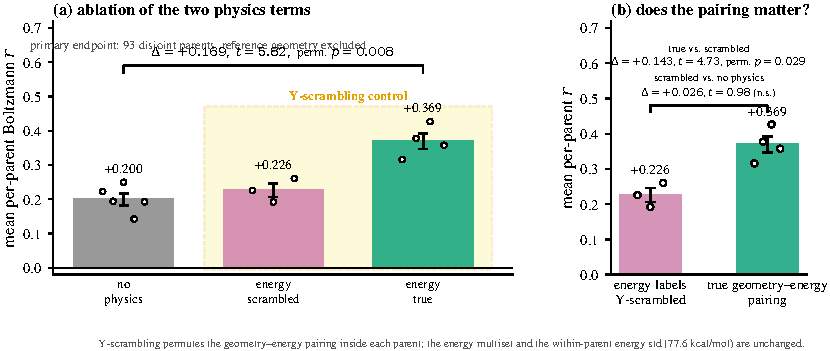
\includegraphics[width=\linewidth]{figures/out/fig3_ablation_bars.pdf}
\end{center}
\caption{Per-seed evidence behind the label ablation of \Cref{sec:ablation}, on the
\textbf{primary endpoint} --- 93 parents disjoint from the energy term's shard pool, scored on
the 8 displaced geometries with the unperturbed reference excluded. Bars are means over
independently trained seeds, error bars are the standard error over seeds, and every seed is an
open circle, because at three or four seeds the raw points are more informative than the
interval. \textbf{(a)} The three arms of the main evaluation round: no physics, energy
supervision with the geometry--energy pairing scrambled inside each parent, and energy
supervision with the true pairing. The bracket is the primary contrast,
$\Delta = +0.169$, Welch $t = 5.82$, exact permutation $p = 0.008$. \textbf{(b)} The same
scrambling pair enlarged: true against scrambled gives $\Delta = +0.143$, $t = 4.73$,
permutation $p = 0.008$, while scrambled against no physics is not significant
($\Delta = +0.024$, $t = 0.80$). Scrambling permutes which energy is attached to which
geometry within a parent, so the energy multiset and the within-parent energy spread
($77.6$~kcal/mol) are bit-for-bit unchanged. Two defects of that control are recorded in
\Cref{sec:ablation} and \Cref{app:data}, and both bias against the contrast shown: only one of
the arm's two shards was scrambled, and its third seed is not configuration-matched.
\emph{What is deliberately absent.} The force cells are not plotted. They come from a
different, smaller round --- $n = 30$ parents, one seed per physics cell, reference geometry
included, and an additional on-policy distillation term --- so they are not comparable with
anything in this figure or in \Cref{tab:boltzmann}; \Cref{tab:cells} reports them with their
only admissible comparator. \emph{What this figure does not show.} It is an ordering
measurement: the scale-sensitive read-outs of the same models are in \Cref{tab:scale}, and they
do not improve.}
\label{fig:ablation}
\end{figure}
